\section{Einführung}
\begin{itemize}
	\item Einsatz hierarchischer DB ab 1970
	\item Relationale DB Einsatz ab 1980; hierarchische DB bleiben bestehen
	\item OO DB Einsatz ab Ende 80er; relationale DB bleiben bestehen
	\item XML DB Einsatz ab 2000; alle alten DB bleiben 
	\item heute: hierarchische DB speichern meisten unternehmenskritischen Daten; gefolgt von Relationalen
	\item OO und XML DB aber in jedem guten relationalen System enthalten
	\item OO DBMS: ab Ende 80er; Startup Unternehmen; komplexes DB-Modell; später unvollkommener, inkonsistenter Standard
	\item Trend OO DBMS: instabil, bei read-write-Transaktionen wenig performant; unvollständig (Zugriffsrechte, Recovery, Sichten, Integritätsbedingungen); verschwinden wieder vom Markt
	\item Objektrelationale DB: Relationale DB integrieren OO Konzepte -> überholen OO DBMS
\end{itemize}

\subsection{Entwicklung der Datenbankmodelle}
Relationenmodell, RDBSs: Objekte dargestellt durch Zeilen in Tabellen
\begin{lstlisting}[mathescape=true]
SET OF RECORD
	$A_1$: Standard-Datentyp$_1$
	...
	$A_n$: Standard-Datentyp$_n$
END;
\end{lstlisting}
\begin{table}[!h]
	\centering
	\begin{tabular}{|l|l|}
		\hline
		Objekttypen	& Eigenschaft\\
		\hline
		\hline
		\textit{Personen}	& \textit{Name} (bestehend aus \textit{Vor}- und \textit{Nachname})\\
							& \textit{Adresse} (bestehend aus \textit{PLZ}, \textit{Ort}, \textit{Straße} und \textit{Hausnummer})\\
							& \textit{Hobbies} (bestehend aus einer Menge von \textit{Hobbies})\\
							& \textit{Geburtsdatum}\\
		\hline
	\end{tabular}
	\caption{Beispiel: Modellierung von Personen}
\end{table}

In RDBS:
\begin{itemize}
	\item Eigenschaften \textit{Name, Adresse} in Komponenten zerlegen
	\item Eigenschaft \textit{Hobbies} auslagern (1NF)
	\begin{table}[!h]
		\centering
		\begin{tabular}{|l|l|l|l|l|l|l|}
			\hline
			Vorname & Nachname & PLZ & Ort & Straße & Hausnr & Gebdat\\
			\hline
			\hline
			&&&&&&\\
			\hline
		\end{tabular}
		\vspace{1cm}
		\begin{tabular}{|l|l|l|l|l|}
			\hline
			Vorname & Nachname & PLZ & Gebdat & Hobby\\
			\hline
			\hline
			&&&&\\
			\hline
		\end{tabular}
	\end{table}
	
	\item Eigenschaften \textit{Vorname, Nachname, PLZ} und \textit{Geburtsdatum} sollen Schlüssel sein
\end{itemize}

\textbf{Eigenschaften relationaler DB}
\begin{itemize}
	\item Starre Strukturen (Relationenschemata)
	\item Einfache Strukturen (nur Tabelle, 1NF)
	\item Für einfache Attributwerte (Zahlen, Zeichenketten, also Standard-Datentypen)
	\item Mit fester Semantik (Built-in Funktionen für Std-Typen)
	\item Austausch von Daten (etwa im Web) erschwert: Trennung Schema (Relationenschema) und Instanz (Relation), zum Versand muss beides zusammengefasst werden
\end{itemize}

\textbf{Entwicklung: OO DB}
\begin{itemize}
	\item Forschung Ende 80er, Hype 90er => Nischenprodukt für neue Anwendungen; Ende 90er in RDBS
	\item Konzepte: komplexe Strukturen (statt nur Tabellen nun auch beliebig strukturierte Objekte)\\
	Komplexe Attributwerte (Typen können konstruiert werden)\\
	mit variabler Semantik (Methoden können def. werden)
\end{itemize}

\textbf{Entwicklung: XML DB}
\begin{itemize}
	\item Forschung 90er, Hype Anfang 00er => Nischenprodukt für bestimmte Anwendungen; XML-Konzepte im objekrelationalen SQL-Standard
	\item Konzepte: Ausgangspunkt Dokumentbeschreibungssprache (Markup-Sprache) statt starrer Datenstruktur\\
	Variable Strukturen zur Beschreibung von Daten und Dokumente\\
	Komplexe Strukturen mit variabler Semantik mgl\\
	Austauschformat im Web zum Dokument- und Datenaustausch
\end{itemize}

\textbf{Entwicklung: Digitale Bibliotheken (ab 2000)}
\begin{itemize}
	\item XML-Dokumente (oder andere Dokumentformate, pdf, doc... oft textlastig) langfristig speichern
	\item Auffindbar machen über strukturierte Metadaten (etwa in XML oder im relationalen DB-Modell)
	\item Spezielle Anforderungen: Dokumente haben Wert, können gekauft werden (E-Commerce)\\
	Dokumenten weltweit eindeutig identifiziert\\
	Identifier sind persistent, nicht flüchtig, obwohl Dokument vergriffen oder gesperrt sein kann\\
	Versionierung der Dokumente
	
	\item Suche nach Features in Texten (Stichworte,..) oder nach strukturierten Metadaten
\end{itemize}

\textbf{Entwicklung: Multimedia DB (ab 95)}
\begin{itemize}
	\item Dokumente nicht nur textlastig, sondern Bild, Audio, Video, 2D/3D-Geoobjekt,...
	\item Problem: Features sind nicht nu Stichworte, sondern\\
	Bei Bildern: Farben und Farbverteilungen, erkannte Objekte wie Gesichter, Muster, Strukturen,..\\
	Bei Videos: Schnitte, Szenen, Bewegungen,...\\
	Bei Audio: speziell Musik, Melodien, Dynamik, Rhythmus,...\\
	Bei Geoobjekten: Enthaltensein, Schnittflächen,...
\end{itemize}

\textbf{Darstellung komplexer Objekte: OODBS}\\
In OO DBS sind nicht nur Std-Typen für Eigenschaften von Objekten erlaubt, sondern auch wdh Anwendung von Typkonstruktoren.
\begin{lstlisting}
CLASS Personen
	TYPE TUPLE
		(Name: TUPLE
			(Vorname: STRING,
			Nachname: STRING),
		Adresse: TUPLE
			(PLZ: INTEGER,
			Ort: STRING,
			Strasse: STRING,
			Hausnummer: INTEGER),
		Hobbies: SET (Hobby: STRING),
		Geburtsdatum: DATE)
\end{lstlisting}

\textbf{Objektidentität}
\begin{itemize}
	\item RDBS: Schlüsselwerte können sich ändern, Identität eines Objektes geht evtl verloren
	\item OODBS: 
	\begin{itemize}
		\item Objekte ex unabhängig von Werten ihrer Eigenschaften, d.h. Identität bleibt gleich, während sich Eigenschaften ändern
		\item in technischen Anwendungen: teilweise Objekte nicht durch äußere Eigenschaften unterscheidbar (Bsp: Menge von Schrauben gleicher Art)
		\item Entscheidung evtl durch Position, aber nicht durch Namen
	\end{itemize}
\end{itemize}

\textbf{Ist-Hierarchie (Vererbung)}
\begin{itemize}
	\item Fehlt in RDBS; quasi nur über viele Fremdschlüssel simulierbar
	\item OODBS:
	\begin{itemize}
		\item Objekttypen in Vererbungshierarchie mgl
		\begin{lstlisting}
		CLASS Studenten INHERITS Personen
			TYPE TUPLE
				(Matrikelnummer: INTEGER,
				Studienfach: STRING,
				Vater: Personen,
				Mutter: Personen,
				...)
		\end{lstlisting}
		\item Vererbung (Studenten sind spezielle Personen) und Komponentenobjekte (Vater und Mutter sind Personen)
	\end{itemize}
\end{itemize}

\textbf{Methoden statt Host-Prozeduren}
\begin{itemize}
	\item RDBS: spezielle Prozeduren und Funktionen von \textit{außen} aufgesetzt\\
	SQL Ausdruck oder sogar Programm in höheren Programmierspraceh\\
	Bsp: Alter einer Person aus Geburtsdatum: Sicht in SQL auf Basistabelle oder C-Programm mit eingebetteter SQL-Anfrage
	
	\item OODBS: neben Eigenschaften auch die mit ihnen durchführbaren Methoden in die Objekttyp-Definition einkapseln und vererben\\
	Bsp: Alter ist in Definition erklärt (Interface, getrennt davon Impl)
\end{itemize}

\textbf{Dokumente}
\begin{itemize}
	\item Text- oder große Multimediadokumente: groß, unstrukturiert/maximal semistrukturiert, variabel strukturiert (Text nicht immer starr in Kapitel/Abschnitt/...)
	
	\item in RDBS:
	\begin{itemize}
		\item als CLOB oder BLOB (völlig unstrukturiert), Metadaten extrahieren in relationale Tabelle (Autor, Titel, Format, Länge...)
		\item oder \textit{schreddern}: Dokument in kleinste Anteile zerlegen und in relationaler Tabelle speichern mit folgenden Problemen\\
		Relation sieht starre Struktur vor\\
		Relation muss Ordnung der kleinste Anteile bewahren bei der Rekonstruktion des gesamten Dokuments
	\end{itemize}
	
	\item in XML DB:
	\begin{itemize}
		\item von unstrukturiert bis voll strukturiert (auch variabel)
		\item Markup-Sprache für Dokumente geeignet
		\item evtl stark strukturierte Anteile in Relationen gespeichert -> Side Tables
	\end{itemize}
\end{itemize}

\subsection{Nachteile relationaler DB}
\textbf{Komponenten DB-Modell}
\begin{itemize}
	\item \textbf{Strukturell:} Datenstrukturen für Anwendungsobjekte, Konzepte, Modellierung von Beziehungen zw Anwendungsobjekten, Integritätsbedingungen\\
	im Relationenmodell: Relationen (Tabellen) für alles, Schlüssel, Fremdschlüssel
	
	\item \textbf{Operationenteil:} Generische Operationen auf Datenstrukturen und Beziehungen\\
	im Relationenmodell: Relationenalgebra, SQL-Anfragen und SQL-Updates
	
	\item \textbf{Höhere Konzepte:} Metainformationen und objektspezifische Operationen,..\\
	im Relationenmodell: höchstens Data Dictionary, sonst nichts
\end{itemize}

\textbf{Vorteile im Relationenmodell}
\begin{itemize}
	\item \textbf{Strukturteil:} einfache, einheitliche Beschreibung der Anwendungsdaten\\
	Exaktes, mathematisches Fundament
	
	\item \textbf{Operationeteil:}
	\begin{itemize}
		\item Deskriptivität: was, nicht wie; mengenorientiert
		\item Abgeschlossenheit: Ergebnis ist wieder eine Relation
		\item Adäquatheit: alle Konzepte des Strukturteils unterstützt
		\item Optimierbarkeit: System kann selbst schnellere Auswertungsreihenfolge finden
		\item effiziente Impl: jede Operation der Relationenalgebra effizient implementierbar
		\item  Sicherheit: jede syntaktisch richtige Anfrage liefert Ergebnis
		\item Orthogonalität: Alle Operationen beliebig miteinander kombinierbar
	\end{itemize}
\end{itemize}

\textbf{Nachteile Datenmodellierung}
\begin{itemize}
	\item Komplexe Attribute: Wertemengen oder mehrere Komponenten nur über Fremdschlüssel simulierbar
	\item Beziehungen: immer über Fremdschlüssel dargestellt

\end{itemize}

\textbf{Nachteile Datenbankentwurf}
\begin{itemize}
	\item Methoden: 
	\begin{itemize}
		\item Informale Methoden: Entity-Relationship Modell abbilden in Relationenschemata\\
		Schwach bei komplexen Attributen (simuliert über n:m-Beziehungen)
		
		\item Formale Algorithmen: Attribute und Abhängigkeiten bestimmen Relationenschemata\\
		Normalformen, Abhängigkeitstreue, ...\\
		Entwurf ohne Semantik, Abhängigkeiten reichen nicht zur Anwendungsbeschreibung
		
		\item Allgemeine Schwächen: Ergebnis verliert mühsam erfasste Semantik
	\end{itemize}
	
	\item mangelnde Semantik: Beschreibung der Semantik mit Abhängigkeiten zw Attributen (funktional\footnote{Attribute bestimmen eindeutig den Wert anderer Attribute, dann spricht man von funktionaler Abhängigkeit}, mehrwertig)\\
	Reale Bsp komplizierter: CIM-Datenbank, Ventilfeder, Anlasserzahnkranz,.. (was bestimmt sich funktional oder mehrwertig)\\
	vernachlässigt: Verbund- und Inklusionsabhängigkeiten
\end{itemize}

\textbf{Nachteile Anfragesprache}\\
Strukturmangel im Ergebnis\\
Beispiel: Dreifacher Verbund zur Rekonstruktion EINES Buches\\
\\
\textbf{Nachteile Anfrageoperationen}\\
Anfragen an komplexe Attribute
\begin{itemize}
	\item keine Unterstützung komplexer Strukturen in Anfrageformulierung
	\item Notwendigkeit expliziter Verbundoperationen
\end{itemize}

\textbf{Nachteile Update-Operationen}\\
Identifikation der Objekte über sichtbare Schlüssel -> Kein Unterschied zw Umzug, Kauf neues Auto\\
OODBS: Objekte eindeutig identifizierbar -> Unterschied zw Umzug und Autokauf
\begin{figure}[!h]
	\centering
	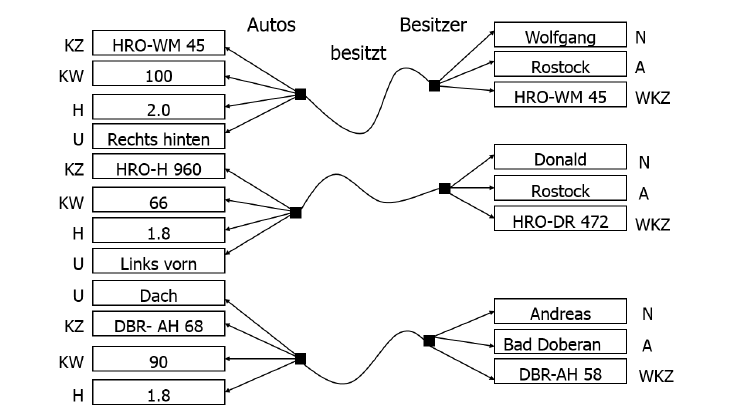
\includegraphics[scale=0.6]{img/object_identity.png}
	\caption{Update Operation in OODBS}
\end{figure}

\textbf{Klassifikation der Probleme}
\begin{itemize}
	\item Art des Problems:\\
	Systemspezifisch (konkret am System, bspw MySQL)\\
	Sprachspezifisch (SQL, jeweiliger Sprachstandard)\\
	Modellspezifisch (liegt am Relationenmodell)
	
	\item Schwere des Problems\\
	Umständlich oder ineffizient (Formulierung von Anfragen)\\
	Zusätzliche Tricks notwendig (Darstellung komplexer Objekttypen)\\
	nicht machbar (bestimmte Arten von Anfragen)
\end{itemize}